
 \chapter{Improving Software Quality}

In this chapter, the basic methodology and activities for improving quality are introduced. Topics include dividing the life cycle of a software into separate periods from the perspective of quality improvement. These periods and the according activities are then described in detail. Unless stated otherwise, the content of this chapter is based on the work of Capers Jones presented in the book The Economics of Software Quality.~\cite{jones2011economics}

% ROI: Three main activities: Review, process audit and testing

\section{Quality Improvement Across the Life Cycle}
\label{sec:life_cycle}


\begin{figure}[t]
\begin{center}
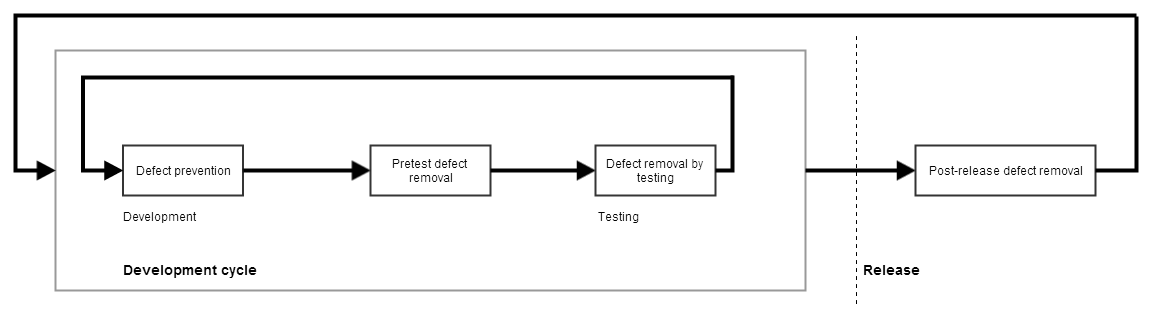
\includegraphics[width=1.0\textwidth]{image/quality_lifecycle.png}
\end{center}
\caption{Phases of software quality improvement in the software life cycle}
\label{fig:quality_life_cycle}
\end{figure}

Quality of a software product can be influenced throughout its life cycle with multiple approaches. Pursuing high quality means having methods in use for both decreasing the amount of defects and maintaining good structural quality. In addition to these technical approaches, projects should have methods to assure high quality of specification and implementation process.

The life cycle of a traditional software project can be divided to periods targeting different quality aspects. The life cycle includes periods concentrating on defect prevention, pretest defect removal, testing and post-release quality improvement as presented in Figure~\ref{fig:quality_life_cycle}. Preventive and pretest periods contain actions such as reviews, inspections and audits. Testing includes various types of testing the functionality. Post-release methods focus on maintainability, defect discovery and defect repairing.

Solid foundation for high quality is built with good specification, requirements and planning in the beginning of a project. When development begins, there should be ways to prevent as much defects as possible. As defects appear anyway, they should be detected and fixed as early as possible. Detecting the defects early lowers the effort needed to fix them. 

The hardest defects to remove are found in the requirements and design because testing and static analysis cannot find them. This is because these defects tend to be deficiency of features and errors of logic rather than errors in code. These defects are usually situated in the beginning of the life-cycle and thus require great effort to be removed. 

At some point, the project can initiate testing phase. Testing is used to systematically find defects in the software. Tests can be aimed to different areas of the software and the range of different tests used is dependent of the project. Big and critical projects should use comprehensive testing whereas smaller projects can get along with smaller amount of tests and lesser coverage.

Quality cannot be forgotten when the software is released. Because defect removal efficiency can never reach 100\%, there are always defects after the release. Some of those defects may have been found in the previous phases, but not removed, and other defects were unknown to the project team at the time of the release. Quality methods after the release should include detecting and removing defects and increasing the design for increasing the maintainability. With this range of methods divided to the software life-cycle, every project should choose the most appropriate methods to be used in the project in question.




 \section{Preventing defects}

Defect prevention is a set of methods used to lower the amount of defects coming from one or many of the defect origins. Software defects are originated from different parts of the project. Defect origins can be technical and nontechnical. Some nontechnical origins of defects include requirements and documentation. Technical origins include architecture, design and code. Because defects are originated from multiple sources, there is no single method for covering them all. Most methods are not effective against all sources. Usually there are 1-4 methods used.

Most of the defect prevention methods are not primarily used for preventing defects, but for some other purpose. Preventing the defects is usually a secondary effect and can be sometimes incidental. These methods don't affect structural quality, but the defects of the software. For achieving high total quality of software, defect prevention should be combined with other types of quality methods.

Defect prevention is one of the most difficult topics of software quality. It is hard to measure, improve and prove the economic value. The difficulty originates from the fact that defect prevention is a negative factor that reduces defect potentials. This means that reliable measurement of the efficiency needs multiple points of reference for both using the method and not using it. Despite this, a number of big companies has studied the topic with significant amounts of projects. IBM, for one example, has been studying this topic since its first studies in 1970s. 

% Inspection

\subsection{Formal Inspections} 
Formal inspections were inspected as a one line of research by IBM in the 1970s. The inspections were targeted at requirements, design documents, source code and other deliverables. In a short time they discovered that the defect removal efficiency with formal inspections could reach levels beyond 85\%. At that time that was higher than any form of testing could achieve. In addition, the inspections seemed to affect the accuracy and completeness of the requirements and specification documents, which lead to raising the defect removal efficiency of testing by 5\%. Combining formal inspections with formal testing could raise the efficiency even further to levels as high as 97\%. 

With these improvements in efficiency, the amount of defects in the beginning of testing was reduced significantly. The schedules and budgets of the testing could be cut to half and in some cases even more than half. That lead to about 15\% decrease in combined schedule and cumulative effort compared to similar applications without inspections.

Another result from the studies was that using the formal inspections for a longer time, the project teams unconsciously started avoiding the kind of errors found in the inspections. This meant that the inspections not only removed defects but also prevented them from occurring.

% TODO: Jotain nykypäivästä?

% Agile development method p.136 / Agile manifesto?
\subsection{Agile Development Method} 
Agile development method is a set of guidelines based on a publication made by 17 software developers. The developers had gathered to discuss about lightweight development methods and the result was the published in The Agile Manifesto. The people in the signature of the manifest formed the Agile Software Development Alliance.

The Agile Manifesto reads as follows:

\begin{quote}

	"Seventeen anarchists agree: 

	We are uncovering better ways of developing software by doing it and helping others do it. Through this work we have come to value: 

	\begin{itemize}
	\item Individuals and interactions over processes and tools.
	\item Working software over comprehensive documentation.
	\item Customer collaboration over contract negotiation.
	\item Responding to change over following a plan.
	\end{itemize}

	That is, while we value the items on the right, we value the items on the left more.

	We follow the following principles:
	\begin{itemize}
	\item Our highest priority is to satisfy the customer through early and continuous delivery of valuable software. 

	\item Welcome changing requirements, even late in development. Agile processes harness change for the customer's competitive advantage. 

	\item Deliver working software frequently, from a couple of weeks to a couple of months, with a preference to the shorter timescale. 

	\item Business people and developers work together daily throughout the project.  
	\item Build projects around motivated individuals. Give them the environment and support they need, and trust them to get the job done. 

	\item The most efficient and effective method of conveying information to and within a development team is face-to-face conversation. 

	\item Working software is the primary measure of progress.  
	\item Agile processes promote sustainable development. The sponsors, developers and users should be able to maintain a constant pace indefinitely. 

	\item Continuous attention to technical excellence and good design enhances agility.  
	\item Simplicity—the art of maximizing the amount of work not done—is essential.  
	\item The best architectures, requirements and designs emerge from self-organizing teams.  
	\item At regular intervals, the team reflects on how to become more effective, then tunes and adjusts its behavior accordingly."

	\end{itemize}

\end{quote}

These methods are based on the actual methods present in the work done by the 17 developers in that time. The purpose of the manifest is not to give definite answers but some guidelines of how to prefer the aspects of software development. It is not trying tell how things are done but help developers with agile methods. When listing the things to value, the purpose is not to underrate the aspects with lower priority but give some hints about what brings the most value to the project.~\cite{beck2001agile}

% TODO: Principlet avattuna paremmin ??????

TODO: Luvut ja faktat 25\% Defect prevention efficiency, 5\% Defect removal efficiency p. 136

% Embedded users p.136 p.58

\textbf{Embedded users.} Embedded users is an Agile method where one or more user representatives are embedded into the project team. The purpose of the user representative is to work in cooperation with the developers creating the critical requirements which are then implemented in short sprints. The idea is to build the specific business critical features and get those running as quickly as possible. The embedded customer representatives are also used to give support in reviewing the features and requirements. The main purpose of this method is to improve the requirements definition.

This method is proven to be useful in small software projects under 2500 function points and effective in projects with under 100 users and size below 1000 function points. In larger scale applications, over 10000 function points or more than 1000 user, a single representative cannot effectively provide enough requirements. This method can however be scaled up by using multiple user representatives, but like other Agile methods, this is most effective in smaller projects.

% Test driven development TDD book?
\subsection{Test-Driven Development} 
Test-driven development (TDD) is a development process where the development consists of short repetitious cycles of development. A cycle comprises an initially failing test case, minimum amount of code to pass that test and refactoring of the code. The development process embraces the phrase "clean code that works" by Ron Jeffries. Kent Beck analyses the benefits of that statement in his book "Test-driven Development: By Example".

Writing clean code that works can help developers by allowing a predictable flow of development. Using tests to define the finished state of a task helps developers know when the task is finished. This is contrary to a common way of development, where developers may be uncertain whether the task is finished or is there still some trail of bugs to fix. Another benefit is that when the developers aims to clean code, instead of building the first thing they think of, they can learn different sides of the problem thinking about another solutions. These benefits lead to enhancing the lives of the users and developers and the whole team. The project team can achieve better trust between the developers and the individual developers can feel better when writing clean code.

Writing clean code that works is not such an easy task. Anyone working in the software development can admit that there are many forces driving the development further from clean code and even from code that works. One solution is using automated tests as the driving force of the development. This is called Test-Driven Development. There are two cornerstones in TDD: new code is written only if an automated test has failed and duplication is eliminated. These rules seem simple enough, but they can actually produce complex behavior for individuals and the whole team. The team must be able to choose between decisions by getting feedback from the running code. Every developer must write his own tests in opposite to waiting for someone else to write the tests. The development environment must be quick enough to provide instant feedback on small changes. The design of the software must allow easy testing by using simple, loosely coupled components.

These complex requirements imply a specific order of activities in development. TDD defines the steps of development and the order of executing them as Red, Green and Refactor. Red and green are the colors of the test success. First a simple test is written so that it won't succeed. The test won't sometimes even compile. Then the test is made green, successful, by not avoiding any means necessary. After the green is achieved, the code is refactored to eliminate all of the duplication created while still keeping the test green.~\cite{beck2003test}


% Static analysis p. 185 (Automated p. 267-276)

\subsection{Static Analysis} 
Static analysis is used to detecting syntactic and structural defects in source code without compiling or executing it. It is used in all sizes of software projects and with every type of applications. The concept is originally from the compilers, which performed syntax checking. Later in the 1970s, the features for detecting defects were improved in a tool called Lint. Static analysis has been further developed over time and nowadays it can comprehensively analyze system-level structure and even security vulnerabilities. Modern tools for static analysis can have defect removal efficiency of over 85\%.

Static analysis tools are based on a library of rules defining the conditions to be examined. Some of the modern commercial tools contain over 1500 rules and allow the users to define their own rules for special conditions. Static analysis is effective in defect removal for using the rules to seek out and eliminate syntactic and structural defects. There are two reasons static analysis is also useful in preventing defects: the rule libraries are also useful for preventing defects and the tools can suggest corrections for defects to the developers. The latter enables the developers to see the effective solutions to the defects while examining the results of the analysis.

Automated static analysis of source code is used in both defect prevention and pretest defect removal. Statistics by Capers Jones show that the usage of automated static analysis exceeds 75\% in most types of software projects. The first mentions of automated static analysis are from 1979 from the first release of Lint. In current modern software development, static source code analysis is automatically done by most of the Integrated Development Environments (IDE). IDEs, such as Eclipse and IntelliJ Idea, perform automatic analysis immediately after every minor change.

Static analysis tools are not only very quick and effective but also fairly inexpensive. Because of this, static code analysis has become one of the most used quality methods in software industry. There are tens or even more tools for source code static analysis in the market, both open source and commercial. For such an inexpensive and effective method, one could imagine the market penetration being close to 100\%. Jones suggests that the reason for this not being true is that humans have a natural resistance for new ideas even though the turn out to be valuable.




% TODO: Summary??

 \section{Pretest Defect Removal}

Capers Jones suggests that in every software project there should be multiple pretest QA methods used. Jones lists a combination of methods for both small and large projects. A small software project, in this context, is described to have a maximum amount of 1000 function points or 50 000 source code statements. These small projects are generally executed by a team with less than 6 software developers. These teams usually have no specialists for any quality methods, but the developers are generalists handling requirements, design, coding and testing. In many cases with Agile approach, there are users representative embedded in the team providing requirements and customers viewpoint in real time. Jones reminds that removing defects with high efficiency requires trained and technically skilled software engineers instead of generalists. However, this is not as necessary in small projects, since fortunately these projects have usually low defect potentials.

\subsection{Origin of Defects}

The origins of defects in small studied projects are split into five categories. Source code is the most common origin of defects. About 1.75 defects per function point are found in source code and this leads to 1750 defects in whole projects. Software design is the second most common source of defects. Design is the origin of 1.00 defects per function point. Requirements are causing 0.75 defects per function point and documentation nearly as much with 0.65 defects. Poorly executed fixes are the origin of 0.27 defects per function point. 

All together these five are the source for 4420 defects in a whole 1000 function point software project. These figures represent the approximate averages and the actual values can be as much as 25\% lower or higher for every source. 

\subsection{Pretest Methods}

Jones presents a suite of pretest defect removal activities and their efficiencies for small projects. This suite includes:

\begin{enumerate}

\item personal desk checking (subsection~\ref{subsec:deskcheck})

\item scrum sessions(subsection~\ref{subsec:scrumsessions})

\item client reviews of specifications(subsection~\ref{subsec:clientreview})

\item informal peer reviews(subsection~\ref{subsec:peerreview})

\end{enumerate}

Each of these forms of defect removal activities are targeted towards a specific type of defects, but other types of defects can be found during the activities. Jones gives several figures for the efficiency of each activity. These figures can only be created by companies that have complete accurate defect measurement programs. Because of this, these figures can vary from context to other and thus are indicative. These figures still illustrate two major problems in the software industry: the removal efficiency levels are comparatively low for most of the removal activities and the defect removal is much harder for requirements and design. The first one leads to a need for numerous kinds of defect removal activities. The latter means that a significant amount of effort must be used to assure the quality of requirements and design. Defects in requirements and design must be removed prior to testing, because the testing cannot find them. Also static analysis is incapable to finding them, because the defects are not bugs found in the code.


% STATSIT: p.198

% Desk checking p. 208
\subsection{Personal Desk Checking} 
\label{subsec:deskcheck}
Personal desk checking is a manual operation in where the logic of an algorithm is checked by the creator of the algorithm . The logic used in the desk checking is presented as a pseudo-code rather than the implemented actual program code. The algorithm is executed by a person acting as a computer. The person performing the desk checking carefully follows the algorithm while filling a table of notes with pen and paper. 

The notes form a table which include columns for: line number, variables in use, conditions, input and output. Line number is necessary to identify the line being executed. All variables have a column in alphabetical order. As the value of the variable changes, the appropriate column is filled up. Conditions columns include a column for every condition in the algorithm which shows the result of the condition in either true (T) or false (F). The condition column is updated whenever the condition is evaluated. Input and output columns are used for the inputs got from the user and the output from the program.~\cite{campionDescCheck}

Desk checking is the oldest form of software defect removal. It has been in use since the beginning of the history of computers. In the early days of computing, testing the programs was difficult because of the limited numbers of computers. The computers worked on production work in the daytime and often the testing had to be done at night. In those days, testing had only an efficiency of 70\% in finding bugs, because of the primitive test case design and limited time available for testing. Therefore the desk checking were a necessary addition to testing. Nowadays the desk checking is still a common activity for removing defects prior to testing. Desk checking today can be enhanced by using static analysis for program code and spell checkers and complexity tools for text documents.

% Figures:
Personal desk checking is used mainly in low-level code. Approximately over 75\% of low-level code and under 30\% of high-level code in projects are checked using personal desk checking. Additionally, personal desk checking is used for over 75\% of text documents, such as requirements. The execution time of desk checking is around 80\% of normal reading speed of text. This leads to about 5 logical statements per minute for source code.

The efficiency of defect removal for personal desk checking is between 25\% and 50\% averaging 35\%. The reason for these relatively low figures can be found in human nature. Humans have a natural tendency to ignore their own mistakes. A developer making an error usually does the error thinking that the action was correct. Therefore when the developer checks the code for defects, the train of thought can remain the same and the defect is not found. This could be avoided by using proofreaders or copy editors, which is a rare habit, but could be profitable for software projects. Another solution for avoiding the blindness to own mistakes is to use peer reviews.


% Scrum sessions p. 222
\subsection{Scrum Sessions} 
\label{subsec:scrumsessions}

The development teams in scrum are usually formed by a scrum master, embedded user representative or stakeholder, possible specialists and three to five developers. In average software development, the team usually has around five software engineers plus one or more specialists as needed. Specialists may include technical writers, business analysts or database specialists. As defined in Agile and scrum, teams should be self-organized and consist of generalists. Thought in many cases having specialized requirements, some specialists are needed.

Projects using Agile and scrum guidelines are split into small units of work. These units are called "sprints" and the development work needed to complete the unit can be achieved in two-week period. The embedded user in the team is responsible to provide the requirements for each sprint. The end result of a sprint should be the source code and supporting documentation ready to be published in production.

One of the principles of scrum is to have daily scrum meetings or "stand ups". The latter name comes from the idea that the people attending the meeting should be standing up so the meeting can stay within the time limit of 15 minutes. During these meetings, every member of the team should describe three things: what was done yesterday, what will be done today and are there any problems that will slow things down. The most interesting topic in the context of defect removal, is listing the issues, bugs and problems there is and simultaneously sharing the knowledge among the team.

Agile and scrum methods are popular and successfully applied in the relatively small, up to 2000 function point in size, projects. In larger software projects, the need for personnel and time raise and the work is more difficult to split in two-week long units. While Agile does have methods for scaling up to larger projects, there are also alternative approaches available.

The statistics by Capers Jones show that Scrum sessions are used in over 90\% of Agile applications and up to 20\% in non-Agile applications. The sessions take under 15 minutes per participant to prepare and optimally not much longer than the limit of 15 minutes per participant to execute. The defect removal efficiency ranges from under 35\% to over 70\% averaging 55\% statistically. However, the statistical efficiency can be somewhat lower than the actual efficiency achieved . This is because the Agile and scrum teams are usually not very strict on collecting the data for defect removal.

% p. 235
\subsection{Client Reviews of Specification} 
\label{subsec:clientreview}

Client reviews of specification are, like the former two methods, among the oldest of defect removal methods. It is still not enough used in average software projects. One of the authors of "The Economy of Software Quality" has got experience in lawsuits for canceled or defective projects. In most of the lawsuits the supplier of the software accuses the customer for failing to review the designs and other documents of not making a remark about any problems during the reviews. In some cases the customer has even accepted the materials quoted in the trial.

The products reviewed by customers usually don't include inner workings of software applications, like source code, test cases or detailed design. Capers Jones presents a list of 12 major items in directly funded software projects, which usually are reviewed:

% TODO: Näihin lause tai pari kuvailemaan tarkoitusta
%	Liekö tarpeellista?

\begin{enumerate}
	\item Requirements.
	\item Requirements changes.
	\item Architecture.
	\item High-level design, user stories, use cases.
	\item Data flow and data structure design.
	\item Development plans.
	\item Development cost estimates.
	\item Development quality estimates.
	\item Training materials.
	\item HELP text and help screens.
	\item Features of COTS packages.
	\item High-severity bug or defect repairs.
\end{enumerate}

Client reviews are an important practice as the clients are paying for the software. There are many clients being active participants in reviews and paying serious attention to the deliverables of software project. Simultaneously some clients are overlooking the reviews and falsely assuming that the software teams know what they are doing. The lawsuits speak on behalf of the reviews, having passive or partial reviews as a worrying feature.

The statistics show that the usage of client reviews of specifications are used in under 50\% of U.S. software applications. The defect removal efficiency varies greatly being at lowest under 15\% and sometimes reaching over 45\%. The average efficiency is around 25\%, which Jones calls "marginally adequate". The effort taken by client reviews is over 2 hours per participant for preparation and over 4 hours per participant for execution. Client reviews work best when the client is directly available, and the applications having indirect clients cannot take full advantage of it.

% Peer review p. 209
\subsection{Peer Reviews} 
\label{subsec:peerreview}

Peer reviews are almost as old as desk checking. The idea of peer reviews is close to the idea of desk checking. The essential difference is that in peer reviews, the code, documentation or other product under review is checked by another person. This prevents the defects from being hidden by the human tendency to ignore their own mistakes. Peer reviews are best suited in small projects with under five developers. 

In larger projects, because of the informal nature of peer reviews, the efficiency of defect removal is better with formal inspections. This leads to informal peer reviews to being the secondary method of defect removal in large projects. In large projects using Agile development method without formal inspections, peer reviews can be highly important.

Peer reviews are targeted to find technical, structural and logical defects. This means that peer reviews are not to be thought as the same as proofreading or copyediting. However, the findings from these can partially overlap each other.

In addition to removing defects in the pretest phase of projects, peer reviews can benefit projects other ways. Peer reviews can achieve the same effect as formal inspections: the participants of the review tend to unconsciously avoid the problems found in the review. Reviews can also be useful for learning. Novice developers can learn while reviewing the work of more experienced developers. Furthermore, experienced developers can remark the problems the novice members need to understand. Even beginner reviewing other beginners work can be better than nothing. Reviews done by expert for the work of expert can be highly efficient, but these cases can sometimes lead to social problems with big egos colliding when mistakes are being pointed out.

Informal peer reviews are used in under a half of software applications. The achieved defect removal efficiency is usually between 35\% and 65\% and the average removal efficiency is 45\%. Reviews can take up to 30 minutes to prepare and the execution pace is around 70\% of the normal reading speed for text, and around 3 logical code statements per minute for source code. Best results for peer reviews can be achieved with small projects using Agile development method.
 

 \section{Testing}

Testing is one of the oldest forms of software defect removal. It has been the most important category of defect removal since the beginning of the software industry, and in many cases even today, it is the only defect removal activity used. Several aspects of testing is covered widely in literature such as testing itself, test case design, test libraries and others. There are also a variety of standards and certifications offered by several companies and groups. Considering the penetration and importance of testing, there is surprisingly low amounts of quantitative data available on testing and test results. Quantitative data in this context means information about numbers of test cases used, numbers of defects found and other information that can be presented in numbers. In addition to the amount of data, the variety of business sizes is not as wide as it could be. The reason for this is that small companies rarely evaluate or benchmark let alone document the results with sufficient precision.

% Definition??

% Quantitive data?? Onko olennaista?


% -Black box / Glass box
% Functional / Nonfunctional
% Automated / Manual
% General / Automatic / Specialized / User
% 
% Testing by developers vs test personnel p.342




 \begin{itemize}
 
 \item Crash, Smoke and Kattava testaus
 
 \item ECO: Chapter 5

 \item ROI: Three main activities: Review, process audit and testing
 
 \end{itemize}

% Test stage frequency p.289
% 
% Average test stages: Subroutine, unit, function, regression, system, beta test
% Defect removal efficiency for these 6 usually 75%-85%. < 1000fp sometimes >90%
% Truly universal: Subroutine and unit tests (+system test with different names)
% 
% p.291 function points vs test stages
% 

% Relevant testing stages for small applications:
% Subroutine testing
% Unit testing?
% New function testing
% Regression testing


 \subsection{Subroutine Testing}

 Subroutine is a small piece of code that may have only a few lines of code. Testing subroutines is the lowest level of testing introduced by Capers Jones. It is a very informal way of testing and is performed almost spontaneously by compiling and executing a subroutine just created. The goal of testing the subroutines immediately after creating them is to verify the correct behavior of the algorithm before the integration of the algorithm to the larger module or application.

 Subroutine testing is a glass box form of testing. It is used in almost every custom-coded software and over 90\% of defect repairs. The defect removal efficiency is between 25\% and 75\% and in average 55\%. Because subroutine testing is such a natural process and is such an efficient way to prevent defects, it is often omitted in testing literature.

 % p.297
 \subsection{Unit Testing}

 Unit testing is aimed at small code modules ranging from around 100 to 1000 source code statements. Units are tested by executing the new or repaired code. In case of developing new features, also the surrounding modules can be unit tested. The testing is usually run by the developer who wrote the module. This leads to poor data collection lowering the amount of data available for unit testing.

 Unit testing contains often bad test cases which are either false positives or not finding defects. When using unit testing, a significant amount of bad fixes and new bugs are introduced while repairing defects.

 The unit testing is often measured by code coverage, the degree of code a certain test suite covers. Aiming for high code coverage is usually a natural objective for test suites, but sometimes a high cyclomatic complexity of the module under test can prevent achieving high coverage. Modules with complexity under 10 can be tested thoroughly but when complexity raises over 20, the removal efficiency of the unit testing will decrease.

 Unit tests can be executed manually but also automatically using a test runner connected to triggers actuating the testing sequence. The usage of automatized unit tests is becoming more common, while the popularity of Continuous Integration systems increase. These systems can be bound to version control systems allowing the automatic execution of tests whenever the source code changes.

 Unit testing is considered as glass box testing. It is used in over 85\% of projects using waterfall and in over 80\% of defect repairs. Unit testing removes from under 25\% to over 55\% and in average cases around 35\% of defects. Unit testing can benefit from the usage of static analysis, which is in most cases performed before the unit testing. In development of complex systems, unit testing can also benefit from code inspections.

% TDD

NOTE! More pollution for testing

 \subsection{New Function Testing}

 \subsection{Regression Testing}

 \subsection{Integration Testing}

 \subsection{System Testing}

 \subsection{Agile Testing}
 
\section{Post Release}

After a software product has been released to the market, it practically always still has defects in it. IBM calls these defects latent defects, because before the release, these defects have not yet been found as problems to customers. The existence of these defects is due to the imperfect effectiveness of the defect removal. Usually the defect removal efficiency is around 85\% and virtually never reaches 100\%.

\subsection{Latent defects}

Some latent defects can be defects found during the development or testing but ones that have not been repaired before the release of the software. Other defects were present in the application, but not discovered by the developers or test personnel. Furthermore, some defects can be originated from new development or other defect repairs in the form of bad fixes. The last two weeks before the release can bring in from about 1\% to even 5\% of delivered defects.

In a traditional development of commercial software, most of the latent defects found in after the release were those that hadn't been found and removed in the development and testing phase. In the more recent history, some vendors have started to release software with remarkable amounts of known, but not removed, defects. In small applications, below 1000 function points, there might be a handful of latent defects present. In larger systems, hundreds of latent defects can be released with the software. Moreover, in massive applications, like Windows 7 or SAP, the amount of known latent defects can sometimes be counted in thousands.

The motivation behind releasing a software with known latent defects appears to be compiled from three factors: first, the aspiration for achieving earlier release dates. Second, an assumption that a quick subsequent release will fix the defects. Third, the utilization of the skills of the customers for finding and repairing defects. The latest of the three can include a strategic offer for customers to get a compensation for repairing or identifying flaws.

This trend of releasing a software knowingly with defects has made customers skeptical about buying or installing the first release of a new software. Some customers prefer to wait for a second release, assuming the latter versions have many of the latent defects removed.
identifying security flaws


\subsection{Defect severity levels}

Because of the potential high amount of defects combined with limited amount of resources for removing them, some system for categorizing the defects on the basis of seriousness is needed. One of the oldest methods for assigning severity levels to defects is the IBM severity scale, which dates back to 1950s. It is still probably the most used severity scale.

The IBM severity scale contains four levels of severities and four other categories of defects. The defects in the first severity level cause that the software does not operate at all. Level 2 defects are disruptions or errors in major features. Level 3 contains minor disruptions, with which the software is still usable. Severity level 4 defects cause cosmetic errors that does not impact the operation of the software.

The other categories in the IBM severity scale consist of four levels existing for convenience. Invalid defect level contains problems that are caused by hardware or other software. Duplicate defect is a category for additional reports of a known defect. Abeyant defect contains defects that cannot be reproduced. Improvement category is for reported defects which are actually suggested improvements.

The usage of the severity scale is for arranging the defects to an order in which they are repaired. Defects in the higher levels are more important to customers than the low-severity defects. Because of this, the group responsible for removing post-release defects use more effort to the higher level defects. The defects in the highest levels may even require temporary fixes to allow the continued usage of the software.

% Structural quality !?!

\subsection{Maintainability}

%Maintainability
%	Maintenance assignment scope
%	Cyclomatic complexity
%	Entropy or rate of structural decay
%
%Positive impact on maintainability
%	Training
%	Structural diagrams
%	Comments clarity
%	No error-prone modules
%	Maintenance tools
%	Maintenance workloads
%	Programming languages
%


\subsection{First year discovery rates}

\subsection{Fixers: Development personnel or Maintenance specialists}

\subsection{Costs of Post-Release Defects in small application}


 

